\chapter{Introduction to Information Systems}

\section{Concept of an Information System}

A database management system (DBMS) is an amalgam of interrelated data and a set of programs designed to access and manipulate said data. The collection of data, termed the \textbf{database}, encapsulates information pertinent to an enterprise or domain of discourse. The paramount objective of a DBMS is to provide a method for the storage and retrieval of information that is both \textbf{convenient and efficient}. \\

The systems under our purview in this treatise deal primarily with \textbf{structured data}. This implies that the data adheres to a pre-defined data model, a formal specification of its organization and relationships. The apotheosis of this paradigm is the relational model, where data is organized into tables (relations) with fixed columns (attributes) and types. This rigid structure facilitates powerful and efficient querying through formal languages like SQL. It is crucial to distinguish this from \textbf{unstructured data} (e.g., text, images, video) or \textbf{semi-structured data} (e.g., XML, JSON), which do not conform to a rigid overall schema. The management of such data has given rise to a different class of systems, often categorized under the NoSQL umbrella (e.g., document stores, key-value stores), which prioritize flexibility and scalability over the strict consistency guarantees of traditional relational systems. Our focus remains on the mathematical elegance and proven robustness of the structured, relational approach.

\begin{mdframed}
\textbf{This is not standard notation, take this just for didactic purposes.}
From another perspective, we can understand an information system $\mathcal{S}$ as a 4-tuple
\[\mathcal{S} = \langle \mathcal{D}, \mathcal{M}, \mathcal{U}, \mathcal{P} \rangle\]
where:
\begin{itemize}
    \item $\mathcal{D}$ is the database, a set of relations $R_1, R_2, \dots, R_n$.
    \item $\mathcal{M}$ is the underlying hardware and network infrastructure.
    \item $\mathcal{U}$ is the set of users and processes that interact with the system.
    \item $\mathcal{P}$ is the set of software, including the operating system and the DBMS.
\end{itemize}

The DBMS acts as a layer of abstraction, concealing the details of the physical implementation and presenting a logical, simplified view of the data.
\end{mdframed}

\section{Components}

\subsection{Users and Processes}
The users of a database system can be classified according to their mode of interaction:
\begin{itemize}
    \item \textbf{Naïve users:} Unsophisticated users who interact with the system by invoking previously written application programs. A clear example is a bank teller using an interface for a transaction.
    \item \textbf{Application programmers:} Computer professionals who develop the application programs.
    \item \textbf{Sophisticated users:} Interact with the system without writing programs, using database query languages to formulate their requests.
    \item \textbf{Database administrators (DBAs):} Individuals responsible for the centralized control of the system. Their functions include schema definition, storage structure and access methods, and the granting of authorizations.
\end{itemize}
A \textbf{process} is an instance of a program in execution that operates on the database.

\subsection{Hardware, Networks, and Client-Server Architecture}
The \textbf{hardware} comprises the physical storage media (main memory, flash storage, magnetic disks) and the processors. Networks, whether local area (LAN) or wide area (WAN), permit communication between different components of the system.

The \textbf{client-server architecture} is a distributed system model in which client processes request services from a server process. In the context of databases, the client (front-end) manages the user interface, while the server (back-end) handles the storage, access, and processing of data. This architecture can be two-tier (client-server) or three-tier (client, application server, database server).

\subsection{Software}
The software component is a hierarchical stack. The two most crucial components that interact directly to bring the database to life are the operating system and the DBMS itself. This shouldn't be a subsection but the syllabus stablishes it in this way.

\subsection{Operating Systems}
The operating system (OS) is the fundamental software layer that manages all hardware resources. It acts as a host for the DBMS. Its importance cannot be overstated, as its performance and functionality impose upper bounds on the performance of the DBMS. The primary functions of the OS in the context of a database system include:
\begin{itemize}
    \item \textbf{Process Management and Scheduling:} The OS manages the concurrent execution of DBMS processes and user application programs, allocating CPU time.
    \item \textbf{Memory Management:} The OS administers main memory (RAM). One of the most critical interactions with the DBMS is the management of the \textit{buffer pool}, an area in main memory where copies of disk blocks are stored to accelerate data access. The efficiency of the OS's page replacement policies (e.g., LRU) directly impacts query performance.
    \item \textbf{Secondary Storage Management:} The OS provides the file system abstraction, hiding the complexity of the disk hardware. The DBMS interacts with this layer to read and write data to persistent storage.
\end{itemize}

While a DBMS can theoretically run on any modern OS, high-performance database servers almost exclusively run on server-grade operating systems. The most dominant choice in the industry is \textbf{Linux} (in its various distributions like Red Hat Enterprise Linux, Ubuntu Server, etc.). This preference is rooted in its open-source nature, unparalleled stability, robust security model, and exceptional performance, particularly in managing memory and I/O operations under heavy loads. \textbf{Windows Server} is also a significant player, especially in enterprise environments deeply integrated with Microsoft's technology stack. Desktop operating systems are fundamentally unsuitable for this task due to their optimization for interactive user experience rather than for the relentless, background service demands of a DBMS.

\subsection{Database Management System}
The Database Management System (DBMS) is the software that defines, manipulates, and manages the database. Its most elegant component is \textbf{data abstraction}, which manifests in a three-level architecture to separate the user's view from the physical implementation.
\begin{description}
    \item[Physical Level:] The lowest level of abstraction, it describes \textit{how} the data is actually stored on the hardware. It defines complex low-level data structures (e.g., B+-trees, hashing) and access methods.
    \item[Logical Level:] The next level of abstraction. It describes \textit{what} data is stored in the database and what relationships exist among that data. This is the level where database administrators (DBAs) define the entire database schema in terms of a data model, such as the relational model. It hides the complexity of the physical level.
    \item[View Level:] The highest level. It allows for the definition of views of the database for individual users. A view is a subset of the database or a restructuring thereof. This level exists to simplify the user's interaction with the system and to provide a security mechanism by hiding parts of the database from certain users.
\end{description}
Furthermore, the DBMS is internally composed of two primary modules: the \textbf{Query Processor} and the \textbf{Storage Manager}.

\subsubsection{Application Programs}
Software designed to interact with the database to perform specific business tasks. These programs communicate with the DBMS through data manipulation languages (like SQL) or application programming interfaces (APIs).

The landscape of relational DBMSs is dominated by a few key systems, each with its distinct mathematical heritage and design philosophy. \textbf{PostgreSQL} is widely revered in academic and professional circles for its strict adherence to the SQL standard and its advanced, object-relational features (this is the one covered in the class). \textbf{MySQL} (and its fork, MariaDB) is ubiquitous in the web development world, prized for its simplicity and speed. In the enterprise sphere, \textbf{Oracle Database} and \textbf{Microsoft SQL Server} are titans, offering comprehensive suites of tools for large-scale data management, analytics, and security. While their interfaces differ, they are all founded upon the relational algebra and calculus proposed by Codd, which we shall explore in due course.

\subsection{Security, Confidentiality, Backup, and Recovery}
\textbf{Security} is addressed as an authorization problem. Modern systems implement sophisticated security models, most commonly \textbf{Role-Based Access Control (RBAC)}. Here, permissions (e.g., select, insert, update on specific tables) are granted to roles, and users are then assigned to these roles. This provides a powerful abstraction that simplifies administration and enhances security over granting permissions to individual users directly.

\textbf{Backup and recovery} are the mechanisms that guarantee the \textit{durability} property of transactions. The most common technique employed is \textbf{write-ahead logging (WAL)}. Before any change is made to the database files on disk, a record of the change is written to a sequential log file. In the event of a crash, the system can replay this log to restore the database to a consistent state, either by redoing committed transactions or undoing incomplete ones. This is complemented by backup strategies:
\begin{itemize}
    \item \textbf{Full backups:} A complete copy of the entire database.
    \item \textbf{Differential backups:} A copy of all data that has changed since the last full backup.
    \item \textbf{Incremental backups:} A copy of all data that has changed since the last backup of any type.
\end{itemize}
Combining these strategies allows for point-in-time recovery (PITR), a critical feature for mission-critical systems.

\textbf{Backup and recovery} are mechanisms to ensure data durability. The system must be able to restore the database to a consistent state after a failure, whether due to a software or hardware fault, or a disaster. This is commonly achieved through periodic backups and a transaction log.

\subsection{Concurrency} %% Update for redirecting to transactions meaning
Concurrency is the ability of the system to allow multiple \textit{transactions} to execute simultaneously. While this improves throughput, it introduces the risk of interference, leading to anomalies such as lost updates or inconsistent reads. The \textbf{concurrency-control} component of the DBMS ensures that such interference does not occur. Its primary goal is to enforce the \textit{isolation} property by ensuring that any execution of concurrent transactions is \textbf{serializable}. A schedule is serializable if it is equivalent (in its effect on the database) to some serial execution of the same transactions. The most common mechanism to achieve this is through \textbf{locking protocols}. In a typical \textbf{two-phase locking (2PL)} protocol, a transaction must acquire a lock on a data item before operating on it and cannot acquire any new locks after it has released one.

\subsection{Database}
Formally, a database can be viewed as a model of a first-order theory. A \textbf{database schema} is the logical design, which acts as the set of axioms of the theory. It defines the relations, their attributes, domains (types), and the integrity constraints. A \textbf{database instance} is the content of the database at a given moment. In logical terms, the instance is a finite structure that is a \textit{model} for the theory defined by the schema. That is, the instance must satisfy all the axioms (constraints). A query, then, is a formula in a logical calculus (like relational calculus), and the result of the query is the set of all tuples that make the formula true within the given model (the instance).

\subsection{Integrity and Consistency}
Data \textbf{integrity} refers to the maintenance and assurance of the accuracy and consistency of data. This is achieved by enforcing \textbf{integrity constraints}, which are the set of predicates or formulas $\Phi$ that any valid database instance must satisfy. A database is in a \textbf{consistent} state if it satisfies all formulas in $\Phi$. Key types of constraints include:
\begin{itemize}
    \item \textbf{Domain Constraints:} Specify that the value of every attribute must be an element from the attribute's domain (e.g., an age must be a positive integer).
    \item \textbf{Entity Integrity:} Enforced by \textbf{primary keys}, this constraint dictates that no attribute of a primary key can be null. This ensures that every tuple in a relation is uniquely identifiable.
    \item \textbf{Referential Integrity:} Enforced by \textbf{foreign keys}, this constraint ensures that a value that appears in one relation for a given set of attributes also appears for a certain set of attributes in another relation. This is the formal mechanism for maintaining consistency between related tables.
\end{itemize}
A transaction, therefore, is an operator that maps one consistent database state to another.

\section{Principal Types of Information Systems}

The fundamental dichotomy in information systems arises from the purpose of data processing. We distinguish between systems optimized for managing ongoing operations and those designed for retrospective analysis and decision-making.

\subsection{Characteristics of Transactional Systems (OLTP)}
Online Transaction Processing (OLTP) systems are engineered to manage operational data. Their primary performance metric is the number of transactions executed per unit of time.
\begin{itemize}
    \item \textbf{Atomicity and Concurrency:} The main focus is handling a large volume of concurrent and relatively simple transactions, ensuring the ACID properties (which will be detailed later).
    \item \textbf{Current Data:} The database represents the \textit{current} state of the domain of discourse. Operations are primarily high-frequency inserts, updates, and deletes on a highly normalized dataset.
    \item \textbf{Simple Queries:} Queries are typically predefined, simple, and affect a small number of records. For instance, querying an account balance or inserting a new order.
    \item \textbf{High Availability:} They require near-100\% availability, as any service interruption directly impacts business operations.
\end{itemize}

\subsection{Characteristics of Analytical Systems (OLAP)}
Online Analytical Processing (OLAP) systems, often associated with Data Warehouses, are optimized for the analysis and aggregation of large volumes of historical data.
\begin{itemize}
    \item \textbf{Historical Orientation:} Data is primarily historical and is loaded into the system periodically (e.g., via ETL - Extract, Transform, Load processes). Update operations are infrequent.
    \item \textbf{Aggregated Data:} Information is organized into multidimensional structures (data cubes) to facilitate analysis. The data is often denormalized to accelerate queries.
    \item \textbf{Complex Queries:} Queries are ad-hoc, complex, and involve the aggregation of millions of records to identify trends, patterns, and anomalies.
    \item \textbf{Massive Data Volume:} They manage data volumes that can be orders of magnitude larger than those of OLTP systems.
\end{itemize}

\section{Transactional Information Systems (OLTP)}

\subsection{The Concept of a Transaction}

From a formal perspective, a transaction is a logical unit of work that must be executed atomically. It is a sequence of operations that transforms the database from one consistent state to another.

\begin{definition}[Transaction]
A transaction $T$ is a finite sequence of operations $\langle o_1, o_2, \dots, o_k \rangle$ on a database $\mathcal{D}$. The execution of $T$ must map a consistent state $\mathcal{D}_i$ to a consistent state $\mathcal{D}_j$. If the transaction cannot be completed in its entirety (commit), the database must be restored to its state prior to the execution of $T$ (rollback).
\end{definition}

\subsection{The ACID Properties of a Transaction}

The ACID properties are a set of axioms that guarantee data integrity even in the face of errors, power failures, or concurrent access. Let $T$ be a transaction:

\begin{itemize}
    \item \textbf{Atomicity:} The transaction is an indivisible unit. Either all operations of $T$ are reflected in the database, or none are. No intermediate states exist. Formally, if $T = \langle o_1, \dots, o_k \rangle$, and $E(T)$ denotes the complete execution of $T$, the final state of the database $\mathcal{D}_{\text{final}}$ is:
    \[ \mathcal{D}_{\text{final}} =
    \begin{cases}
        E(T)(\mathcal{D}_{\text{initial}}) & \text{if } T \text{ succeeds (commits)} \\
        \mathcal{D}_{\text{initial}} & \text{if } T \text{ fails (aborts/rolls back)}
    \end{cases}
    \]

    \item \textbf{Consistency:} The execution of a transaction must preserve the integrity constraints of the database. If the database $\mathcal{D}$ is in a consistent state before $T$, it must also be in a consistent state after its successful execution. Let $\Phi$ be the set of integrity predicates. If $\mathcal{D}_{\text{initial}} \models \Phi$, then $E(T)(\mathcal{D}_{\text{initial}}) \models \Phi$.

    \item \textbf{Isolation:} Concurrent transactions must execute as if they were isolated from one another. The intermediate results of a transaction $T_i$ are not visible to other transactions $T_j$ (with $i \neq j$) until $T_i$ has completed (committed). The concurrent execution of a set of transactions $\{T_1, \dots, T_n\}$ must be equivalent to some serial execution thereof. This concept is formalized by the notion of \textit{serializability}.

    \item \textbf{Durability:} Once a transaction has successfully completed (committed), its effects on the database are permanent and must survive subsequent system failures (e.g., system crashes or reboots). This is guaranteed by mechanisms such as write-ahead logging.
\end{itemize}

\chapter{Analysis, Design, and Implementation of Transactional Information Systems (OLTP)}

The design of a database is a process of successive refinement, moving from an informal, high-level specification of the real world to a precise, implementable, and mathematically sound description. This process is rigorously structured into distinct phases of abstraction.

\section{Requirements Analysis and Conceptual Design}

The initial phase involves capturing user requirements to derive a complete understanding of the data to be stored and the operations that will be performed upon it.

\subsection{Conceptual Design and the E-R Model}
The objective of conceptual design is to produce a high-level data model, independent of any specific DBMS. The Entity-Relationship (E-R) model is the canonical formalism for this task, providing a semantic and graphical language to model the universe of discourse.

\begin{definition}[Entity and Entity Set]
An \textbf{entity} is a distinguishable real-world object. An \textbf{entity set} is a collection of entities of the same type, sharing the same properties, called attributes. E.g., \textit{Professor}.
\end{definition}

\begin{definition}[Relationship and Relationship Set]
A \textbf{relationship} is an association among two or more entities. A \textbf{relationship set} is a mathematical relation on $n \ge 2$ (possibly non-distinct) entity sets. If $E_1, \dots, E_n$ are entity sets, then a relationship set $R$ is a subset of the Cartesian product $\{(e_1, \dots, e_n) | e_1 \in E_1, \dots, e_n \in E_n\}$.
\end{definition}

\noindent\textbf{Constraints} are fundamental to the E-R model:
\begin{itemize}
    \item \textbf{Mapping Cardinalities:} These constrain the number of entities to which another entity can be associated via a relationship set. For a binary relationship set between A and B, common cardinalities are one-to-one (1:1), one-to-many (1:N), and many-to-many (N:M).
    \item \textbf{Participation Constraints:} Specify whether the existence of an entity depends on its being related to another entity via the relationship set. \textbf{Total participation} means every entity in the entity set must participate in at least one relationship. \textbf{Partial participation} means otherwise.
\end{itemize}

An entity set that does not have a primary key is termed a \textbf{weak entity set}. The existence of a weak entity is dependent on a strong entity set, and it must have total participation in the identifying relationship.

\section{Logical Design}

In this phase, the high-level conceptual model is mapped into the implementation data model of a specific DBMS. This is the \textbf{logical model}.

\subsection{The Relational Model}
The relational model, conceived by E. F. Codd, is founded upon set theory and first-order predicate logic.

\begin{definition}[Relation]
A \textbf{relation} consists of two parts:
\begin{itemize}
    \item \textbf{Schema:} Specifies the name of the relation, $R$, and the set of its attributes, $\{A_1, \dots, A_n\}$. For each attribute $A_i$, there is a specified domain, $dom(A_i)$. The schema is denoted $R(A_1, \dots, A_n)$.
    \item \textbf{Instance:} A finite set of \textbf{tuples}. A tuple $t$ is an element of the Cartesian product $dom(A_1) \times \dots \times dom(A_n)$. A relation instance is thus a subset of this product, i.e., $r(R) \subseteq dom(A_1) \times \dots \times dom(A_n)$.
\end{itemize}
\end{definition}

\noindent\textbf{Keys} are a central concept for enforcing integrity:
\begin{itemize}
    \item A \textbf{superkey} is a set of attributes $K \subseteq R$ such that for any two distinct tuples $t_1, t_2$ in any instance of $R$, $t_1[K] \neq t_2[K]$.
    \item A \textbf{candidate key} is a minimal superkey (no proper subset of it is also a superkey).
    \item A \textbf{primary key} is a candidate key chosen by the database designer as the principal means of unique identification.
\end{itemize}

\subsection{Mapping the E-R Model to the Relational Schema}
The process of translating a conceptual E-R diagram into a logical relational schema is not an art but a systematic, algorithmic procedure. Following this algorithm ensures that all entities, relationships, and constraints are faithfully represented in the relational model. The standard textual notation for a relational schema is:
\texttt{RELATION\_NAME(pk\_attribute1, pk\_attribute2, attribute3, ..., fk\_attributeN (FK), ...)}

\begin{description}
    \item[Step 1: Mapping Strong Entity Sets] For each strong entity set $E$ in the E-R model, create a relation (table) $R$ that includes all the simple attributes of $E$. The primary key of the relation $R$ is the primary key of the entity set $E$.
    \begin{itemize}
        \item \textit{Example:} An entity set \texttt{SCHOOL} with attributes \texttt{school\_id} (primary key) and \texttt{location} becomes: \\
        \texttt{School(\underline{school\_id} integer, location varchar(100))}
    \end{itemize}

    \item[Step 2: Mapping Weak Entity Sets] For each weak entity set $W$ with an identifying strong entity set $S$, create a relation $R_W$. The attributes of $R_W$ include all simple attributes of $W$. The primary key of $R_W$ is a composite key consisting of the primary key of $S$ and the discriminator of $W$. A foreign key is also established from $R_W$ referencing $S$.
    \begin{itemize}
        \item \textit{Example:} A weak entity \texttt{Building} identified by \texttt{School} with discriminator \texttt{building\_name} becomes: \\
        \texttt{Building(\underline{school\_id (FK)}, \underline{building\_name}, capacity integer)}
    \end{itemize}

    \item[Step 3: Mapping Relationship Sets] The mapping of a relationship set depends on its cardinality.
    \begin{itemize}
        \item \textbf{Many-to-Many (N:M):} For each N:M relationship set $R$ between entity sets $E_1$ and $E_2$, create a new relation $R_{12}$. The primary key of $R_{12}$ is the composite of the primary keys of $E_1$ and $E_2$. Any descriptive attributes of the relationship set become attributes of this new relation.
        \begin{itemize}
        \item \textit{Example:} A many-to-many relationship \texttt{STUDIES\_IN} between \texttt{Student} and \texttt{School} becomes: \\
        \texttt{StudiesIn(\underline{student\_curp (FK)}, \underline{school\_id (FK)}, education\_level varchar(50))}
        \end{itemize}
        \item \textbf{One-to-Many (1:N):} Do not create a new relation. For a 1:N relationship between $E_1$ (the "one" side) and $E_2$ (the "many" side), take the primary key of $E_1$ and include it as a foreign key attribute in the relation for $E_2$.
        \begin{itemize}
        \item \textit{Example:} A one-to-many relationship where one \texttt{School} has many \texttt{Students}: \\
        \texttt{Student(\underline{student\_curp}, student\_name, school\_id (FK))}
        \end{itemize}
        \item \textbf{One-to-One (1:1):} Similar to 1:N, but the choice of where to place the foreign key is more flexible. It can be placed in either relation. To avoid nulls, it is often placed in the relation corresponding to the entity set with total participation in the relationship.
    \end{itemize}

    \item[Step 4: Mapping Attributes]
    \begin{itemize}
    \textit{ }
        \item \textbf{Composite Attributes:} These are flattened. For a composite attribute $A$ composed of sub-attributes $A_1, \dots, A_n$, create distinct attributes for each sub-attribute in the corresponding relation.
        \item \textbf{Multi-valued Attributes:} For a multi-valued attribute $M$ of an entity set $E$, create a new relation $R_M$. This relation will have a composite primary key consisting of the primary key of $E$ and an attribute corresponding to $M$.
        \begin{itemize}
        \item \textit{Example:} A professor can have multiple phone numbers: \\
        \texttt{ProfessorPhone(\underline{prof\_id (FK)}, \underline{phone\_number})}
        \end{itemize}
    \end{itemize}
\end{description}
This deterministic procedure ensures a complete and correct translation from the conceptual to the logical model, producing a schema ready for normalization and implementation.

\subsection{Database Normalization}
Normalization is the process of decomposing relation schemas to minimize data redundancy and avoid update anomalies (insertion, deletion, modification anomalies). It is based on the concept of \textbf{functional dependencies}.

\begin{definition}[Functional Dependency (FD)]
Let $R$ be a relation schema, and let $\alpha, \beta$ be subsets of the attributes of $R$. The functional dependency $\alpha \to \beta$ holds on $R$ if for all pairs of tuples $t_1, t_2$ in any legal instance of $R$, if $t_1[\alpha] = t_2[\alpha]$, then it must be that $t_1[\beta] = t_2[\beta]$. This means the values of the attributes in $\alpha$ uniquely determine the values of the attributes in $\beta$.
\end{definition}

\noindent The process of normalization is a progression through a series of \textbf{normal forms}:
\begin{itemize}
    \item \textbf{First Normal Form (1NF):} This is the foundational axiom of the relational model. A relation is in 1NF if the domain of every attribute contains only \textbf{atomic} values. The term "atomic" signifies that the values are indivisible from the perspective of the DBMS.

    \begin{remark}
    Explicitly... Let $t$ be an arbitrary tuple in any instance of a relation schema $R(A_1, \dots, A_n)$. The schema is in 1NF if for any attribute $A_i$, the value $t[A_i]$ is an element of a domain $dom(A_i)$ that is not a composite structure.

    A domain is defined as composite if it can be expressed as an $n$-ary Cartesian product of other domains, $D_1 \times D_2 \times \dots \times D_n$ for $n > 1$, or as the power set $\mathcal{P}(D)$ of some base domain $D$.
    \begin{itemize}
        \item \textbf{Prohibition of Composite Attributes:} A domain structured as a Cartesian product would permit values that are themselves tuples, violating atomicity. For example, a domain $D_{\text{Name}} = D_{\text{First}} \times D_{\text{Last}}$ is non-atomic.
        \item \textbf{Prohibition of Multi-valued Attributes:} A domain structured as a power set would permit values that are sets of values, such as $\{ \text{v}_1, \text{v}_2, \dots \}$, also violating atomicity.
    \end{itemize}
    Therefore, enforcing 1NF is equivalent to stipulating that for every attribute, its domain cannot be decomposed into such products or power sets from the perspective of the data model. This indivisibility is a prerequisite for the algebraic properties of the relational model.
    \end{remark}
    
    \item \textbf{Second Normal Form (2NF):} A relation is in 2NF if it is in 1NF and every non-prime attribute (an attribute not part of any candidate key) is fully functionally dependent on every candidate key. This form is mainly of historical interest.
    \item \textbf{Third Normal Form (3NF):} A schema $R$ is in 3NF if for every FD $\alpha \to \beta$ that holds on $R$, at least one of the following is true:
    \begin{enumerate}
        \item $\beta \subseteq \alpha$ (it is a trivial dependency).
        \item $\alpha$ is a superkey for $R$.
        \item Each attribute in $\beta - \alpha$ is contained in a candidate key of $R$.
    \end{enumerate}
    This form eliminates transitive dependencies on the key.
    \item \textbf{Boyce-Codd Normal Form (BCNF):} A schema $R$ is in BCNF if for every FD $\alpha \to \beta$ that holds on $R$, at least one of the following is true:
    \begin{enumerate}
        \item $\beta \subseteq \alpha$ (it is a trivial dependency).
        \item $\alpha$ is a superkey for $R$.
    \end{enumerate}
\end{itemize}
\begin{remark}
BCNF is a stricter form than 3NF. Every relation in BCNF is also in 3NF. However, a relation in 3NF is not necessarily in BCNF. While BCNF is theoretically more desirable as it eliminates more anomalies, sometimes a decomposition to achieve BCNF might fail to preserve all functional dependencies. Therefore, 3NF is often considered the acceptable standard for transactional database design, representing a pragmatic trade-off between eliminating redundancy and preserving dependencies.
\end{remark}

\subsection{Relational Algebra}
Relational algebra is a procedural query language that forms the theoretical foundation for relational databases and query languages like SQL. It is a closed algebra, where the operands are relations and the result of every operation is itself a relation.

\noindent\textbf{Fundamental Set-Theoretic Operations:}
These operations are inherited directly from set theory, requiring that the operand relations $R$ and $S$ be \textbf{union-compatible} (i.e., they have the same arity and the domains of their corresponding attributes are identical).
\begin{itemize}
    \item \textbf{Union ($R \cup S$):} Forms a relation containing all tuples that appear in $R$, or in $S$, or in both.
    \item \textbf{Set Difference ($R - S$):} Forms a relation containing all tuples that appear in $R$ but not in $S$.
    \item \textbf{Cartesian Product ($R \times S$):} Forms a relation from all possible concatenations of a tuple from $R$ with a tuple from $S$. If $R$ has arity $k_1$ and $S$ has arity $k_2$, the result has arity $k_1+k_2$. It is the foundation upon which all meaningful joins are built.
\end{itemize}

\noindent\textbf{Fundamental Relational Operations:}
\begin{itemize}
    \item \textbf{Select ($\sigma_{p}(R)$):} A horizontal filter. It produces a relation containing only the tuples from $R$ that satisfy the selection predicate $p$. Formally, $\sigma_{p}(R) = \{t \in R \ | \ p(t) \text{ is true}\}$.
    \item \textbf{Project ($\Pi_{\alpha}(R)$):} A vertical filter, as discussed above. Given a set of attribute names $\alpha$, it produces a relation containing tuples constructed from the specified attributes in $R$, with duplicates eliminated.
    \item \textbf{Rename ($\rho_{x(B_1, \dots, B_n)}(E)$):} An essential operator for clarity and avoiding ambiguity, especially in complex expressions involving self-joins. It renames the relation produced by expression $E$ to $x$, and its attributes to $B_1, \dots, B_n$.
\end{itemize}

\begin{remark}[On Projections]
There is a curious connection between relational projection and its namesake in linear algebra. In a vector space, a projection operator $\Pi: V \to W$ maps a vector onto a subspace $W$, effectively reducing its dimensionality by discarding components orthogonal to $W$.

In the relational model, a relation can be viewed as a set of vectors (obviously the cartesian product of atributes is not a vector space, but tuples can be compeared as them) in a space whose basis vectors are the attributes. The relational projection operator $\Pi_{A_1, \dots, A_k}(R)$ is precisely analogous. It is a transformation that maps the set of tuples onto a lower-dimensional subspace defined by the basis vectors (attributes) $A_1, \dots, A_k$. The other "dimensions" (attributes) are discarded. The final step of eliminating duplicate tuples ensures the result adheres to the set-theoretic foundation of the model. This is not a mere terminological coincidence; it is a manifestation of the same fundamental mathematical idea of dimensionality reduction.
\end{remark}

\noindent\textbf{The Taxonomy of Join Operations:} Joins are derived operations, but they are the most critical for combining information. They are fundamentally composed of a Cartesian product followed by a selection. The variety of joins reflects different ways of specifying the selection criteria and handling non-matching tuples.

\begin{itemize}
    \item \textbf{Theta Join ($R \bowtie_{\theta} S$):} The most general form. It selects tuples from the Cartesian product that satisfy a predicate $\theta$. It is formally defined as: $R \bowtie_{\theta} S = \sigma_{\theta}(R \times S)$.
    \item \textbf{Equijoin:} A specific case of the Theta Join where the predicate $\theta$ consists solely of equalities.

    \item \textbf{Natural Join ($R \bowtie S$):} The most frequently used join. It is an equijoin on all attributes that are common to both $R$ and $S$. The common attributes appear only once in the resulting relation. It is a composition of product, selection, and projection.

    \item \textbf{Outer Joins:} These joins extend the natural join to preserve tuples that do not have a match in the other relation, padding the missing attributes with NULL values. This prevents information loss.
    \begin{itemize}
        \item \textbf{Left Outer Join ($R \leftthreetimes S$):} Includes all tuples from the natural join, plus all tuples from $R$ that did not match any tuple in $S$, padded with NULLs for the attributes of $S$.
        \item \textbf{Right Outer Join ($R \rightthreetimes S$):} The symmetric counterpart to the left outer join, preserving non-matching tuples from $S$.
        \item \textbf{Full Outer Join ($R \fullouterjoin S$):} Preserves non-matching tuples from both $R$ and $S$, padding with NULLs where appropriate. It is the union of the left and right outer joins.
    \end{itemize}

    \item \textbf{Semijoins:} These are not true joins in that they do not combine attributes from both tables. Instead, they act as powerful filters.
    \begin{itemize}
        \item \textbf{Left Semijoin ($R \ltimes S$):} Returns only the tuples from $R$ for which there is at least one matching tuple in $S$ (based on the common attributes). The schema of the result is identical to the schema of $R$. Formally: $R \ltimes S = \Pi_{Schema(R)}(R \bowtie S)$.
        \item \textbf{Right Semijoin ($R \rtimes S$):} The converse, returning tuples from $S$ that have a match in $R$.
    \end{itemize}

    \item \textbf{Antijoins:} The logical opposite of a semijoin.
    \begin{itemize}
        \item \textbf{Left Antijoin ($R \triangleright S$):} Returns tuples from $R$ for which there is \textit{no} matching tuple in $S$. The schema of the result is identical to the schema of $R$. Formally: $R \triangleright S = R - (R \ltimes S)$.
    \end{itemize}
\end{itemize}

\noindent\textbf{Division Operation ($\div$):}
The division operator is designed for queries that involve universal quantification (i.e., "for all"). Let the schemas be $R(A,B)$ and $S(B)$. The expression $R \div S$ returns a relation over the attributes $A$ containing all tuples $t_A$ from $R$ such that for every tuple $t_S$ in $S$, the tuple $\langle t_A, t_S \rangle$ is in $R$. It can be expressed using the fundamental operators:
\[ R \div S = \Pi_{A}(R) - \Pi_{A}((\Pi_{A}(R) \times S) - R) \]

\section{Physical Design}
Physical design is the final phase in the database design process, concerned with the actual storage of data on a physical medium. While logical design describes \textit{what} data is stored, physical design specifies \textit{how} this data is stored and accessed. The primary objective is to optimize performance for the expected workload.

Key decisions in the physical design phase include:
\begin{itemize}
    \item \textbf{File Organization:} Determining the physical arrangement of data records on disk. Common strategies include heap file organization (records placed in no particular order) and sequential file organization (records stored in sequential order based on a search key).
    \item \textbf{Indexing:} The creation of auxiliary data structures to accelerate data retrieval. An index on an attribute allows the DBMS to locate tuples with a specific value for that attribute without scanning the entire relation. The most prevalent index structure in relational databases is the \textbf{B+-tree}.
    \item \textbf{Data Partitioning:} The technique of splitting a large table into smaller, more manageable pieces (partitions) while preserving the logical unity of the table. This can be done horizontally (by rows) or vertically (by columns) to improve query performance and system manageability.
\end{itemize}
Although modern DBMSs automate many physical design decisions, a foundational understanding of these principles is indispensable for performance tuning and database administration.

\section{SQL: The Standard Relational Language}
Structured Query Language (SQL) is the standard language for interacting with relational database management systems. It is fundamentally a declarative language, where the user specifies the desired state or result, and the DBMS query optimizer determines the most efficient procedural execution plan. SQL is comprised of several sublanguages for distinct tasks.

\subsection{Data Definition Language (DDL)}
The DDL is used to define and manage the database schema. Its commands create, modify, and destroy the relational structures themselves. While the most granular work occurs at the table level, the highest-level container for all objects is the database itself.

\begin{description}
    \item[Create Database (Idempotent)] This command creates a new, independent database. A database is a named collection of schemas and other objects. To ensure scripts are re-runnable without error, the \texttt{if not exists} clause is used. This makes the operation \textbf{idempotent}: it guarantees the existence of the database after execution, regardless of its prior state, without raising an error if it already exists. This is the first command one must execute when starting a new project.
    \begin{minted}[fontsize=\small, frame=single, framesep=5pt, linenos]{sql}
Create database if not exists vibenotes_db;
    \end{minted}
    The counterpart is drop if exists, its usage is trivial.
\end{description}

% The \subsubsection{Data Types} and subsequent sections follow immediately after this block.

\subsubsection{Data Types}
Every attribute must be assigned a data type, which defines its domain of permissible values, its storage representation, and the set of operations that can be applied to it. A robust understanding of these types is critical for schema design, ensuring both data integrity and storage efficiency.

\begin{description}
    \item[Character Types] Used for storing strings of text. The fundamental distinction lies in their storage allocation:
    \begin{itemize}
        \item \texttt{char(n)}: A fixed-length character string, blank-padded to exactly \textit{n} characters. It is suitable for data with a known, consistent length, such as ISO country codes.
        \item \texttt{varchar(n)}: A variable-length character string with a specified maximum length of \textit{n}. It uses only the storage required for the actual string, making it efficient for data of varying lengths.
        \item \texttt{text}: A variable-length character string of effectively unlimited length, intended for large bodies of text.
    \end{itemize}

    \item[Numeric Types] These are divided into exact and approximate types.
    \begin{itemize}
        \item \textbf{Exact Numerics:} Store values with perfect precision. This category includes \texttt{integer} (typically 32-bit), \texttt{bigint} (typically 64-bit), and \texttt{numeric(p,s)} or \texttt{decimal(p,s)}. The \texttt{numeric} type is paramount for financial and scientific calculations, storing a number with a total of \textit{p} digits (\textbf{precision}) and \textit{s} digits after the decimal point (\textbf{scale}).
        \item \textbf{Approximate Numerics:} These are floating-point types, such as \texttt{real} and \texttt{double precision}. They are subject to rounding errors and are unsuitable for applications where exactness is required (e.g., financial accounting).
    \end{itemize}

    \item[Monetary Types] Some systems, like PostgreSQL, offer a non-standard \texttt{money} type. While convenient, it is often vendor-specific and may have fixed-precision limitations. The formally correct and portable approach for handling currency is to use the standard \texttt{numeric(p,s)} type, which provides explicit control over precision and scale, thereby preventing rounding errors.

    \item[Temporal Types] For storing date and time information.
    \begin{itemize}
        \item \texttt{date}: Stores the year, month, and day.
        \item \texttt{time}: Stores the hour, minute, and second, often with fractional precision.
        \item \texttt{timestamp}: Stores both date and time. The SQL standard defines variants such as \texttt{timestamp with time zone} to handle temporal data unambiguously across different geographic locations.
    \end{itemize}

    \item[Boolean Type] Represents the truth values of classical logic. The SQL \texttt{boolean} type can hold values \texttt{true}, \texttt{false}, or \texttt{null}. The presence of \texttt{null} elevates the system's logic from a two-valued logic to a three-valued logic, where \texttt{null} represents an "unknown" or "missing" truth value.
\end{description}

\subsubsection{Schema and Constraint Definition}
The primary DDL command is \texttt{create table}, which defines a relation, its attributes, and its integrity constraints.
\begin{itemize}
    \item \textbf{Primary Key:} Uniquely identifies each tuple in a relation. Implies \texttt{unique} and \texttt{not null}.
    \item \textbf{Foreign Key:} A foreign key is a set of attributes in a relation whose values are required to match the values of a candidate key in some other (or the same) relation. Its purpose is to enforce \textbf{referential integrity}, a logical constraint ensuring that relationships between tables remain consistent. A state of referential integrity exists if for every non-null foreign key value, a corresponding primary key value exists in the referenced table. This prevents the existence of "orphan" records with invalid references.

When an operation (like \texttt{delete} or \texttt{update}) attempts to modify a referenced primary key, the DBMS must ensure referential integrity is maintained. The \texttt{on delete} and \texttt{on update} clauses allow the schema designer to specify the precise policy for maintaining this consistency automatically.

\begin{description}
    \item[\texttt{cascade}] This policy enacts a cascading deletion. When a referenced tuple is deleted, all tuples that reference it are also recursively deleted. This models a strong \textit{compositional} or \textit{ownership} relationship, where the existence of the referencing entities is dependent on the existence of the referenced entity. For example, deleting a specific \texttt{Invoice} should cascade to delete all its associated \texttt{LineItem} entries.

    \item[\texttt{set null}] This policy severs the link without deleting the referencing tuple. When a referenced tuple is deleted, the foreign key columns in all referencing tuples are set to \texttt{null}. This models a weaker, optional association, implying that the referencing entity can exist independently of the referenced one. This policy requires that the foreign key column(s) be nullable. For instance, if a \texttt{Professor} leaves a \texttt{Department}, their record might remain while their `dept\_id` is set to \texttt{null}.

    \item[\texttt{restrict} / \texttt{no action}] This is the most conservative and often default policy. It rejects any operation that would violate referential integrity. The deletion of a referenced tuple is blocked if any tuples reference it. This forces an explicit resolution of the dependencies (e.g., by manually reassigning or deleting the referencing tuples) before the parent tuple can be removed.
\end{description}
    \item \textbf{Not Null:} Ensures an attribute cannot have a \texttt{null} value.
    \item \textbf{Unique:} Ensures all values in a column or set of columns are unique.
    \item \textbf{Check:} Specifies a predicate that every tuple in the relation must satisfy.
\end{itemize}

\begin{minted}[fontsize=\small, frame=single, framesep=5pt, linenos]{sql}
Create table Department (
    dept_id   integer,
    dept_name varchar(255) not null unique,
    budget    numeric(12, 2) check (budget > 0),
    primary key (dept_id)
);

Create table Professor (
    prof_id      integer,
    first_name   varchar(255) not null,
    dept_id      integer,
    primary key (prof_id),
    foreign key (dept_id) references Department(dept_id) on delete set null
);
\end{minted}

\subsubsection{Index Management}
Indexes are redundant data structures that improve the speed of data retrieval operations, at the cost of slower writes and increased storage. B+-Trees are the most common index implementation.
\begin{minted}[fontsize=\small, frame=single, framesep=5pt, linenos]{sql}
Create index prof_dept_idx on Professor(dept_id);
\end{minted}

\subsubsection{Post-Creation Schema Modification and Predicate Operators}
Integrity constraints are not immutable; they can be added, removed, or modified on existing relations using the \texttt{alter table} command. This allows the logical schema to evolve over time. Furthermore, the predicates used in \texttt{check} constraints and \texttt{where} clauses are not limited to simple arithmetic comparisons; SQL provides a rich set of operators for pattern matching and more complex logical tests.

\begin{description}
    \item[Modifying Constraints] The \texttt{alter table} statement is the primary mechanism for all schema modifications after a table has been created.
    \begin{itemize}
        \item \textbf{Adding a Constraint:} New constraints can be given a user-defined name for easier reference.
        \begin{minted}[fontsize=\small, frame=single, framesep=5pt, linenos]{sql}
-- Adds a check constraint to the Professor table
alter table Professor
add constraint check_prof_id_positive check (prof_id > 0);
        \end{minted}

        \item \textbf{Dropping a Constraint:} Constraints are removed by referencing the name they were given.
        \begin{minted}[fontsize=\small, frame=single, framesep=5pt, linenos]{sql}
alter table Professor
drop constraint check_prof_id_positive;
        \end{minted}
    \end{itemize}

    \item[Predicate Syntax and Operators] The power of \texttt{check} constraints and \texttt{where} clauses is derived from a wide array of available operators.
    \begin{itemize}
        \item \textbf{Standard Comparison:} The standard operators include \texttt{=} (equality), \texttt{<>} or \texttt{!=} (inequality), \texttt{<}, \texttt{<=}, \texttt{>}, \texttt{>=}.
        \item \textbf{Pattern Matching (\texttt{like}):} Provides simple pattern matching for strings. The underscore (\texttt{\_}) matches any single character, and the percent sign (\texttt{\%}) matches any sequence of zero or more characters. The \texttt{ilike} variant is case-insensitive.
        \begin{minted}[fontsize=\small, frame=single, framesep=5pt, linenos]{sql}
-- Finds names starting with 'T' and ending with 'g'
select first_name from Professor where first_name like 'T%g';
        \end{minted}
        \item \textbf{POSIX Regular Expressions:} For more complex pattern matching, PostgreSQL provides operators based on POSIX regular expressions. These offer a far more powerful and expressive syntax than \texttt{like}.
        \begin{itemize}
            \item \texttt{\~}: Case-sensitive match.
            \item \texttt{\~\*}: Case-insensitive match.
            \item \texttt{!\~}: Case-sensitive non-match.
            \item \texttt{!\~\*}: Case-insensitive non-match.
        \end{itemize}
        \begin{minted}[fontsize=\small, frame=single, framesep=5pt, linenos]{sql}
-- Finds names that start with a vowel (case-insensitive)
select first_name from Professor where first_name ~* '^[aeiou]';
        \end{minted}
    \end{itemize}
\end{description}

\subsubsection{Data Retrieval and Join Operations}
The \texttt{select} statement is the cornerstone of data retrieval. While its basic form filters a single relation, its true power is unleashed when combining information from multiple relations. This is achieved through \texttt{join} clauses, which are the practical, syntactic implementations of the relational algebra's powerful join operators. A join operation constructs a composite result set from the tuples of two or more relations based on a specified logical predicate.

Let us consider two relations for our examples: \texttt{Professor(prof\_id, prof\_name, dept\_id)} and \texttt{Department(dept\_id, dept\_name)}.

\begin{description}
    \item[Inner Join] This is the most common join operation. It returns only the tuples for which the join predicate evaluates to true. It effectively computes the intersection of the two relations based on the join condition. Tuples from either relation that do not have a matching tuple in the other are excluded from the result.

    \begin{center}
    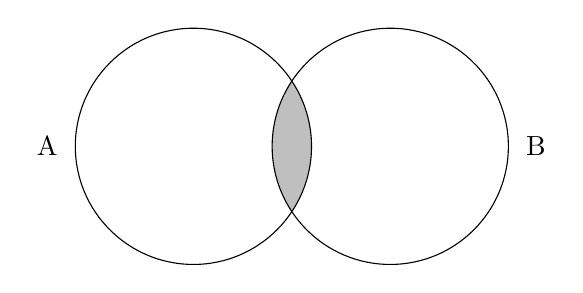
\begin{tikzpicture}
        \begin{scope}
            \clip (0,0) circle (1.5cm);
            \fill[gray!50] (2.5,0) circle (1.5cm);
        \end{scope}
        \draw (0,0) circle (1.5cm) node[left=1.6cm] {A};
        \draw (2.5,0) circle (1.5cm) node[right=1.6cm] {B};
    \end{tikzpicture}
    \end{center}

    \begin{minted}[fontsize=\small, frame=single, framesep=5pt, linenos]{sql}
Select p.prof_name, d.dept_name
from Professor as p
inner join Department as d on p.dept_id = d.dept_id;
    \end{minted}

    \item[Natural Join] This is a syntactic simplification of an inner join. A \texttt{natural join} implicitly joins the two relations on all attributes that share the same name. The common columns appear only once in the result set. While convenient, it can be dangerous in complex schemas where column names might match coincidentally, leading to incorrect results. Explicit joins with an \texttt{on} clause are formally preferred for clarity and safety.

    \begin{minted}[fontsize=\small, frame=single, framesep=5pt, linenos]{sql}
-- This is equivalent to the inner join above, because both tables
-- share only the `dept_id` column.
select prof_name, dept_name
from Professor
natural join Department;
    \end{minted}

    \item[Left Outer Join (or Left Join)] This join returns all tuples from the left relation, along with the matched tuples from the right relation. If a tuple in the left relation has no corresponding match in the right relation, the attributes from the right relation are populated with \texttt{null}.

    \begin{center}
    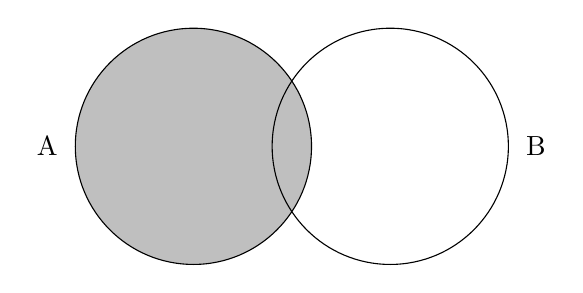
\begin{tikzpicture}
        \fill[gray!50] (0,0) circle (1.5cm);
        \draw (0,0) circle (1.5cm) node[left=1.6cm] {A};
        \draw (2.5,0) circle (1.5cm) node[right=1.6cm] {B};
    \end{tikzpicture}
    \end{center}

    \begin{minted}[fontsize=\small, frame=single, framesep=5pt, linenos]{sql}
-- This query would list all professors, including those
-- whose dept_id is null or does not exist in the Department table.
Select p.prof_name, d.dept_name
from Professor as p
left join Department as d on p.dept_id = d.dept_id;
    \end{minted}

    \item[Right Outer Join (or Right Join)] The logical symmetric of the left join. It returns all tuples from the right relation, along with the matched tuples from the left relation. If a tuple in the right relation has no corresponding match in the left, the attributes from the left relation are populated with \texttt{null}.

    \begin{center}
    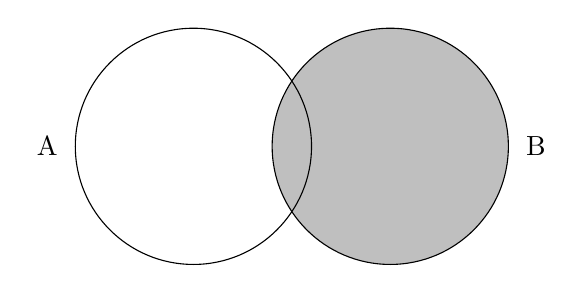
\begin{tikzpicture}
        \fill[gray!50] (2.5,0) circle (1.5cm);
        \draw (0,0) circle (1.5cm) node[left=1.6cm] {A};
        \draw (2.5,0) circle (1.5cm) node[right=1.6cm] {B};
    \end{tikzpicture}
    \end{center}

    \begin{minted}[fontsize=\small, frame=single, framesep=5pt, linenos]{sql}
-- This query would list all departments, including those
-- that currently have no professors assigned to them.
Select p.prof_name, d.dept_name
from Professor as p
right join Department as d on p.dept_id = d.dept_id;
    \end{minted}

    \item[Full Outer Join] This join synthesizes the behavior of the left and right outer joins. It returns all tuples from both relations, matching them where possible and populating non-matching attributes with \texttt{null}. It represents the set-theoretic union of the datasets with respect to the join condition.

    \begin{center}
    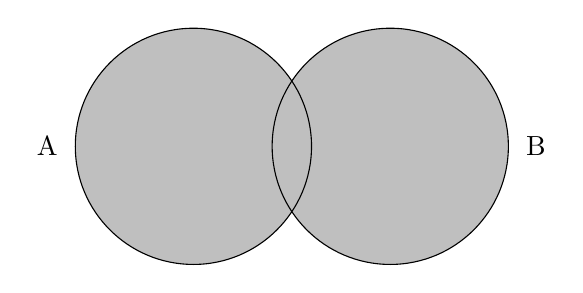
\begin{tikzpicture}
        \fill[gray!50] (0,0) circle (1.5cm);
        \fill[gray!50] (2.5,0) circle (1.5cm);
        \draw (0,0) circle (1.5cm) node[left=1.6cm] {A};
        \draw (2.5,0) circle (1.5cm) node[right=1.6cm] {B};
    \end{tikzpicture}
    \end{center}
    
    \begin{minted}[fontsize=\small, frame=single, framesep=5pt, linenos]{sql}
-- This query lists all professors and all departments, matching
-- them where possible and preserving all non-matching entities.
Select p.prof_name, d.dept_name
from Professor as p
full outer join Department as d on p.dept_id = d.dept_id;
    \end{minted}

     \item[Excluding Join (Anti-Join)] This is not a distinct join type but a crucial logical pattern used to find tuples in one relation that have no match in another. It implements the set difference operation. The general principle is to perform an outer join and then filter the result set in the \texttt{where} clause, keeping only those rows where the key from the non-preserved table is \texttt{null}, which signals a failed match.

    \begin{center}
    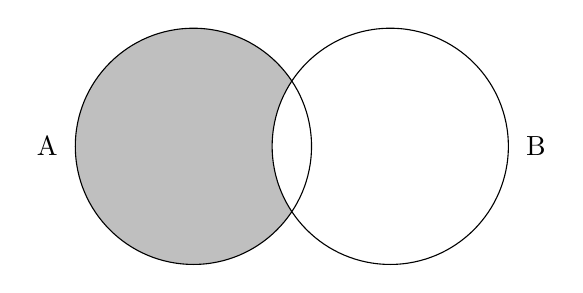
\begin{tikzpicture}
        \begin{scope}
            \clip (0,0) circle (1.5cm);
            \fill[gray!50] (0,0) circle (1.5cm);
            \fill[white] (2.5,0) circle (1.5cm);
        \end{scope}
        \draw (0,0) circle (1.5cm) node[left=1.6cm] {A};
        \draw (2.5,0) circle (1.5cm) node[right=1.6cm] {B};
    \end{tikzpicture}
    \end{center}

    \begin{minted}[fontsize=\small, frame=single, framesep=5pt, linenos]{sql}
-- This query finds all professors who are NOT assigned to a valid department.
-- It returns the set A - B.
Select p.prof_name
from Professor as p
left join Department as d on p.dept_id = d.dept_id
where d.dept_id is null;
    \end{minted}

    \item[Cross Join] This join returns the Cartesian product of the two relations. Every tuple from the left relation is combined with every tuple from the right.
    
    \begin{remark}
    A Venn diagram is an inappropriate visual metaphor for a Cross Join. Venn diagrams illustrate set intersection and union. A Cross Join is a Cartesian product, an operation that generates a new set of ordered pairs whose dimensionality is the sum of the dimensionalities of the input sets, which cannot be represented by overlapping planar regions.
    \end{remark}

    \begin{minted}[fontsize=\small, frame=single, framesep=5pt, linenos]{sql}
-- This query returns a row for every possible pairing of a
-- professor and a department, regardless of their actual association.
Select p.prof_name, d.dept_name
from Professor as p
cross join Department as d;
    \end{minted}
\end{description}

\subsubsection{Aggregation, Filtering, and Ordering}
Beyond joining relations, the true analytical power of SQL lies in its ability to aggregate data, filter those aggregations, and order the final results for presentation. These capabilities are handled by the \texttt{group by}, \texttt{having}, and \texttt{order by} clauses.

\begin{description}
    \item[Aggregation (\texttt{group by})] The \texttt{group by} clause partitions the tuples of a relation into groups, such that all tuples in a given group have the same values for the grouping attributes. Aggregate functions (\texttt{count}, \texttt{sum}, \texttt{avg}, \texttt{min}, \texttt{max}) are then applied to each group to compute a summary value.

    \textbf{Relational Algebra Equivalent:} This operation is represented by the generalized aggregation operator, $\mathcal{G}$ (Gamma). Its form is:
    \[ \mathcal{G}_{G_1, ..., G_m, F_1(A_1), ..., F_k(A_k)}(R) \]
    Here, $G_1, ..., G_m$ are the attributes on which to group. For each group, the functions $F_1, ..., F_k$ are applied to the attributes $A_1, ..., A_k$. The resulting relation contains the grouping attributes and the results of the aggregate functions.

    \item[Group Filtering (\texttt{having})] The \texttt{having} clause is used to filter the \textit{groups} created by the \texttt{group by} clause. This is fundamentally different from the \texttt{where} clause, which filters individual tuples \textit{before} aggregation. The \texttt{having} predicate can only contain conditions on the grouping attributes or on aggregate functions.

    \textbf{Relational Algebra Equivalent:} A \texttt{having} clause corresponds to a selection operation ($\sigma$) that is applied \textit{after} the aggregation operator $\mathcal{G}$.
    \[ \sigma_{P}(\mathcal{G}_{...}(R)) \]
    Where $P$ is the predicate of the \texttt{having} clause.

    \item[Ordering (\texttt{order by})] The \texttt{order by} clause is used to sort the final result set based on the values of one or more attributes, in ascending (\texttt{asc}) or descending (\texttt{desc}) order.

    \textbf{Relational Algebra Equivalent:} The pure relational model is based on set theory, and sets are inherently unordered. Therefore, there is no ordering operator in the classic relational algebra. However, to model the behavior of SQL, an extended algebra often includes a sorting operator, $\tau$ (Tau), which is applied as the final operation.
    \[ \tau_{A_1, ..., A_n}(R) \]
    This operator is not part of the standard formal algebra but is a practical extension to represent the presentation layer of a query.
\end{description}

\begin{remark}[The Chronology of a Complete Query]
A complete SQL query is a syntactic representation of a deeply nested composition of relational algebra operators. The logical order of execution is crucial and differs from the written order of the clauses.
\end{remark}

Consider the following query, which finds departments with more than 10 professors and a total budget exceeding \$5,000,000, ordered by department name:
\begin{minted}[fontsize=\small, frame=single, framesep=5pt, linenos]{sql}
select
    d.dept_name,
    count(p.prof_id) as professor_count
from Department as d
inner join Professor as p on d.dept_id = p.dept_id
where d.budget > 5000000
group by d.dept_name
having count(p.prof_id) > 10
order by d.dept_name asc;
\end{minted}

This query is logically equivalent to the following complete compositional expression in extended relational algebra, which reveals the true execution chronology:

\begin{equation*}
\begin{split}
\tau_{\text{dept\_name}} \left( \Pi_{\text{dept\_name, professor\_count}} \left( \sigma_{\text{professor\_count} > 10} \left( \mathcal{G}_{\text{dept\_name, count(prof\_id) as professor\_count}} \right. \right. \right. \\
\left. \left. \left. \left( \sigma_{\text{budget} > 5000000} \left( \text{Department} \bowtie_{\text{dept\_id}} \text{Professor} \right) \right) \right) \right) \right)
\end{split}
\end{equation*}

This formal expression shows the precise sequence of operations:
\begin{enumerate}
    \item \textbf{Product/Join:} The relations are joined. (\texttt{from}, \texttt{join})
    \item \textbf{Tuple Selection:} Individual tuples are filtered. (\texttt{where})
    \item \textbf{Grouping \& Aggregation:} The surviving tuples are partitioned and aggregated. (\texttt{group by})
    \item \textbf{Group Selection:} The resulting groups are filtered. (\texttt{having})
    \item \textbf{Projection:} The final attributes for the result set are selected and named. (\texttt{select})
    \item \textbf{Ordering:} The final result set is sorted for presentation. (\texttt{order by})
\end{enumerate}

\subsection{Data Control Language (DCL)}
The DCL is concerned with security, managing user permissions via roles and privileges.
\begin{minted}[fontsize=\small, frame=single, framesep=5pt, linenos]{sql}
Grant select on Professor to some_role;
Revoke update on Department from some_user;
\end{minted}

\subsection{Stored Procedures and Functions}
Most modern DBMSs allow for the creation of stored procedures and functions, which are blocks of procedural code (often in a dialect of SQL like PL/pgSQL for PostgreSQL) stored within the database. This allows complex logic to be executed on the server, reducing network traffic and ensuring consistent application of business rules.

\begin{minted}[fontsize=\small, frame=single, framesep=5pt, linenos]{sql}
-- A PostgreSQL function to add a new professor
Create function add_professor(p_id integer, p_name varchar, p_dept integer)
returns void as $$
begin
    insert into Professor(prof_id, first_name, dept_id)
    values (p_id, p_name, p_dept);
end;
$$ language plpgsql;
\end{minted}

\subsection{Interacting with a PostgreSQL Server}
Practical interaction with a database server is a two-stage process. First, a secure connection to the host machine must be established. Second, the database client is invoked from within that secure session to execute commands, either interactively or via a script.

\subsubsection{Establishing a Secure Shell (SSH) Connection}
Before interacting with the database, a secure, encrypted channel to the server must be opened using the Secure Shell (SSH) protocol.
\begin{minted}{bash}
ssh -p 2206 alumno##@132.248.51.117
\end{minted}
The components of this command are:
\begin{itemize}
    \item \texttt{ssh}: The command to initiate the SSH client.
    \item \texttt{-p 2206}: Specifies a non-standard port for the connection.
    \item \texttt{alumno\#\#}: The username for the account on the remote server.
    \item \texttt{132.248.51.117}: The IP address of the target server.
\end{itemize}
Upon successful authentication, you will be granted a command-line shell on the remote server.

\subsubsection{Interactive Session with psql}
Once connected via SSH, the standard PostgreSQL client, \texttt{psql}, can be used for interactive sessions.

\noindent To connect, one typically uses:
\begin{minted}{bash}
psql -U username -d database_name
\end{minted}
The \texttt{psql} environment provides meta-commands for inspecting the database schema:
\begin{itemize}
    \item \texttt{\textbackslash l}: Lists all available databases.
    \item \texttt{\textbackslash dt}: Lists all tables in the current database's default schema.
    \item \texttt{\textbackslash d table\_name}: Describes the specified table.
    \item \texttt{\textbackslash q}: Quits the \texttt{psql} session.
\end{itemize}

\subsubsection{Script Creation and Execution}
For any non-trivial work, executing commands from a script is the superior, reproducible method. The \texttt{vim} text editor is a standard, powerful tool for this on Linux systems.

\begin{description}
    \item[Creating a Script:] A new SQL script can be created and edited using \texttt{vim}:
    \begin{minted}{bash}
vim my_script.sql
    \end{minted}
    Inside \texttt{vim}, one would enter SQL commands (e.g., \texttt{create table...}, \texttt{insert into...}).

    \item[Executing a Script:] The script can be executed directly by the \texttt{psql} client using input and output redirection from the main server shell.
    \begin{minted}{bash}
psql -U username -d database_name < my_script.sql > output.txt
    \end{minted}
    This command has three parts:
    \begin{itemize}
        \item \texttt{psql -U ... -d ...}: Invokes the client with connection details.
        \item \texttt{< my\_script.sql}: This is \textbf{input redirection}. It instructs the shell to feed the contents of \texttt{my\_script.sql} into the standard input of the \texttt{psql} client, executing the commands within.
        \item \texttt{> output.txt}: This is \textbf{output redirection}. It instructs the shell to capture all standard output from the \texttt{psql} command (query results, notices, etc.) and write it to the file \texttt{output.txt}, rather than displaying it on the screen.
    \end{itemize}
\end{description}
This scripted, non-interactive approach is essential for version control, automation, and maintaining a verifiable record of all database operations.

\subsection{Codd's Twelve Rules}
In his seminal work, E. F. Codd observed that many systems claiming to be "relational" were merely storing data in tables without adhering to the underlying mathematical principles of the model. To provide a rigorous benchmark, he published a set of rules to define what constitutes a truly relational database management system (RDBMS). A system's adherence to these rules is a measure of its relational fidelity.

\begin{description}
    \item[Rule 0: The Foundation Rule] For a system to be a true RDBMS, it must manage the database entirely through its relational capabilities.
    
    \item[Rule 1: The Information Rule] All information in a relational database—including user data and metadata—is to be represented explicitly and solely in one way: as values in tables.
    \[ \forall \text{info } i, \exists R \in \mathcal{D}, \exists t \in R, \exists A \in \text{Attributes}(R) \text{ s.t. } i = t[A] \]

    \item[Rule 2: The Guaranteed Access Rule] Every single datum (atomic value) must be logically accessible by resorting to a combination of table name, primary key value, and attribute name.
    \[ \forall t \in R \in \mathcal{D}, \forall A \in \text{Attributes}(R), \exists! v \text{ s.t. } v = \text{lookup}(R, t[K_R], A) \]

    \item[Rule 3: Systematic Treatment of Null Values] Null values, distinct from empty strings or zero, must be supported for representing missing or inapplicable information in a systematic way, independent of data type.
    \[ \forall A, \text{dom}(A) \supseteq \{\text{NULL}\} \]

    \item[Rule 4: Dynamic On-Line Catalog Based on the Relational Model] The database description (catalog), $\mathcal{C}$, is represented at the logical level in the same way as ordinary data, allowing authorized users to apply the same relational language, $\mathcal{L}$, to its query.
    \[ \mathcal{C} \subseteq \mathcal{D} \quad \land \quad \forall R_c \in \mathcal{C}, \text{query}(R_c, \mathcal{L}) \text{ is valid} \]

    \item[Rule 5: The Comprehensive Data Sublanguage Rule] A relational system must support at least one well-defined language, $\mathcal{L}$, that is comprehensive in its support for all database operations (DDL, DML, DCL, etc.).
    \[ \exists \mathcal{L} : \mathcal{L} \to \{\text{DDL, DML, DCL, TCL}, ...\} \]

    \item[Rule 6: The View Updating Rule] All views that are theoretically updatable must be updatable by the system. For a view $V = f(R_1, ..., R_k)$, if $f$ is invertible:
    \[ \forall \text{update } U(V), \exists U'(R_1,...,R_k) \text{ s.t. } U(V) \equiv f(U'(R_1,...,R_k)) \]

    \item[Rule 7: High-Level Insert, Update, and Delete] The system must support set-at-a-time \texttt{insert}, \texttt{update}, and \texttt{delete} operators. Operations act on relations, not individual tuples.
    \[ \forall \text{op} \in \mathcal{L}_{\text{DML}}, \text{op}: \mathcal{P}(\text{Tuples}) \to \mathcal{P}(\text{Tuples}) \]

    \item[Rule 8: Physical Data Independence] Application programs remain logically unimpaired whenever changes are made in storage representations or access methods. Let $q$ be an application query.
    \[ \text{PhysicalRepr}(R) \to \text{PhysicalRepr}'(R) \implies q(R) \text{ is unchanged} \]

    \item[Rule 9: Logical Data Independence] Application programs remain logically unimpaired when information-preserving changes are made to the base tables. Let $R \to R'$ be an info-preserving change.
    \[ \forall q \text{ not referencing changed attributes}, q(R') \text{ is valid and yields } q(R) \]

    \item[Rule 10: Integrity Independence] Integrity constraints, $\Phi$, must be specified separately from application programs and stored in the catalog.
    \[ \Phi \subset \mathcal{C} \quad \land \quad \Phi \text{ is independent of application code} \]

    \item[Rule 11: Distribution Independence] The data manipulation sublanguage must enable applications to operate successfully even if data is physically distributed.
    \[ q(\mathcal{D}_{\text{distributed}}) \equiv q(\mathcal{D}_{\text{centralized}}) \]

    \item[Rule 12: The Nonsubversion Rule] If the system provides a low-level language, $\mathcal{L}_{\text{low}}$, it must not be possible to use it to subvert the integrity constraints, $\Phi$, expressed in the higher-level language.
    \[ \nexists \text{ op} \in \mathcal{L}_{\text{low}} : (\mathcal{D}_1 \models \Phi) \to (\mathcal{D}_2 \not\models \Phi) \]
\end{description}

\subsection{The Relational and In-Memory Models for Transactional Systems}
For Online Transaction Processing (OLTP) systems, where data integrity, consistency, and high throughput of atomic operations are paramount, the relational model is the optimal paradigm. Its rigorous foundation in set theory, strong consistency guarantees via the ACID transaction properties, and the elimination of data anomalies through normalization make it uniquely suited for these applications.

However, as transactional workloads have intensified, the performance bottleneck has shifted to the physical I/O of traditional disk-based storage. The state-of-the-art solution to this is the \textbf{in-memory database}. Such systems store the entire operational dataset within main memory (RAM), virtually eliminating disk I/O latency for data reads. This results in an orders-of-magnitude increase in transaction processing speed. Durability is not sacrificed; it is ensured by writing transaction logs to persistent storage and creating periodic snapshots of the in-memory state.

The synthesis of the relational model's logical rigor with the performance of in-memory storage represents the pinnacle of modern architecture for high-performance transactional systems.